\documentclass[11pt]{article}

% Change "review" to "final" to generate the final (sometimes called camera-ready) version.
% Change to "preprint" to generate a non-anonymous version with page numbers.
\usepackage[review]{acl}

% Standard package includes
\usepackage{times}
\usepackage{latexsym}
\usepackage[table]{xcolor}
\usepackage{placeins}
\usepackage{tabularx}
\usepackage{booktabs}

% For proper rendering and hyphenation of words containing Latin characters (including in bib files)
\usepackage[T1]{fontenc}
% For Vietnamese characters
% \usepackage[T5]{fontenc}
% See https://www.latex-project.org/help/documentation/encguide.pdf for other character sets

% This assumes your files are encoded as UTF8
\usepackage[utf8]{inputenc}

% This is not strictly necessary, and may be commented out,
% but it will improve the layout of the manuscript,
% and will typically save some space.
\usepackage{microtype}

% This is also not strictly necessary, and may be commented out.
% However, it will improve the aesthetics of text in
% the typewriter font.
\usepackage{inconsolata}

%Including images in your LaTeX document requires adding
%additional package(s)
\usepackage{graphicx}
\usepackage{float}

% If the title and author information does not fit in the area allocated, uncomment the following
%
%\setlength\titlebox{<dim>}
%
% and set <dim> to something 5cm or larger.

\title{Relational Grounding Failures in Zero-Shot Cross-Lingual Dialogue Summarization with Small Language Models}

\author{
Yunwoo Lee, Jennifer Huang, Ziwa Li \\
Department of Linguistics, University of Washington, Seattle, WA, USA \\
\texttt{\{yunu919, jjnhuang, lizhihua\}@uw.edu}
}

\begin{document}
\maketitle
\raggedbottom
\begin{abstract}
We diagnose relational grounding failures in zero-shot English-to-Chinese dialogue summarization with small language models (SLMs). We develop and apply a Dialogue-Semantic Grounding Error Taxonomy to evaluate three open-weight SLMs alongside a supervised mBART baseline. The taxonomy captures errors in entities, events, speaker roles, circumstances, modality, discourse outcomes, omissions, and language or format. Our analysis shows that SLM hallucinations are often relational rather than arbitrary: models preserve dialogue-relevant content while altering who did what, under what conditions, or with what outcome. These findings position the taxonomy as a diagnostic tool for dialogue summarization, revealing relation-sensitive faithfulness failures that reference-based metrics may obscure.
\end{abstract}

\section{Introduction}
Small language models (SLMs) are attractive for resource-constrained, industrial, and privacy-sensitive summarization because they are more efficient and locally deployable than large language models \citep{abrougui-etal-2026-small,xu-etal-2025-evaluating,philippy-etal-2025-enhancing}. In cross-lingual dialogue summarization, a model generates a target-language summary from a source-language dialogue. However, it remains unclear whether SLMs can produce summaries that are not only fluent, but also faithfully grounded in the source dialogue. In this work, a summary is faithful only if its entities, events, speaker roles, circumstances, modality, and discourse outcomes are supported by the dialogue.

We study this question through zero-shot English-to-Chinese dialogue summarization, where models must identify salient events and speaker roles in English and express the result in Chinese \citep{wang-etal-2022-clidsum,wang-etal-2023-zero}. Prior work shows that cross-lingual summarization is sensitive to dataset construction, translation artifacts, and evaluation design \citep{bhattacharjee-etal-2023-crosssum,wang-etal-2023-understanding}, but automatic metrics alone may obscure how outputs fail to preserve dialogue meaning.

Prior work has proposed fine-grained factual-error taxonomies for dialogue summarization, including errors involving wrong references, circumstances, negation, tense, modality, subject/object relations, pronouns, particulars, and hallucinations \citep{tang-etal-2022-confit,wang-etal-2022-analyzing}. Building on this work, we propose a source-grounded, relation-sensitive diagnostic framework for cross-lingual dialogue summarization. Our Dialogue-Semantic Grounding Error Taxonomy reorganizes overlapping error phenomena around entities, events, participant roles, circumstances, modality, and discourse relations, while also covering salient omissions and cross-lingual language or output-form failures. Using this taxonomy alongside ROUGE, BERTScore, and OmniScore, we compare open-weight SLMs with a supervised mBART baseline and show that SLM hallucinations are often relational: models may preserve dialogue-relevant content while misrepresenting who did what, under what conditions, or with what outcome.


\begin{table}[H]
\centering
\scriptsize
\setlength{\tabcolsep}{2pt}
\renewcommand{\arraystretch}{0.92}
\begin{tabularx}{\columnwidth}{@{}lX@{}}
\toprule
Label & Core annotation trigger \\
\midrule
\textsc{H-Ent} & Wrong or unsupported person, entity, name, or object. \\
\textsc{H-Evt} & Added, changed, or fabricated event/action. \\
\textsc{H-Role} & Correct event but wrong actor, recipient, speaker, or role. \\
\textsc{H-Circ} & Wrong time, place, number, quantity, condition, or schedule. \\
\textsc{H-Mod} & Changed negation, uncertainty, intention, obligation, or modal force. \\
\textsc{H-Disc} & Misstated cause-effect, contrast, order, decision, agreement, conclusion, or outcome. \\
\textsc{Omit} & Missing salient event, participant, reason, decision, or outcome. \\
\textsc{Lang} & English leakage, malformed Chinese, repetition, translation/format issue, or non-summary output. \\
\textsc{No-Error} & No grounding, omission, language, format, or instruction-following error. \\
\bottomrule
\end{tabularx}
\caption{Dialogue-Semantic Grounding Error Taxonomy. \textsc{H-*} labels indicate hallucination; \textsc{Omit} and \textsc{Lang} capture missing content and output-form failures.}
\label{tab:taxonomy}
\end{table}

\section{Experimental Setup}
\subsection{Data}

We evaluate models on XSAMSum, a cross-lingual dialogue summarization dataset from the ClidSum benchmark \citep{wang-etal-2022-clidsum}, which extends the English SAMSum corpus \citep{gliwa-etal-2019-samsum} with professional summaries in multiple target languages. We focus on English-to-Chinese summarization, where models generate Chinese summaries from English messenger-style dialogues. For diagnostic evaluation, we use a fixed random sample of 100 test examples from the XSAMSum test split selected with seed 42. Dataset and evaluation-subset statistics are reported in Appendix~\ref{sec:appendix-data}.


\subsection{Models}

We compare a supervised mBART-large-50 baseline \citep{liu-etal-2020-multilingual-denoising,tang-etal-2021-multilingual} with three open-weight instruction-tuned SLMs under 10B parameters: Aya Expanse 8B \citep{dang2024ayaexpansecombiningresearch}, Gemma 4 E4B \citep{gemma4_2026}, and Qwen 3.5 9B \citep{qwenteam2026qwen35omnitechnicalreport}. The mBART baseline is fine-tuned on the XSAMSum training data, while the SLMs are evaluated in a zero-shot direct setting. Given an English dialogue, each SLM is prompted to generate a concise Simplified Chinese summary. The same prompt is used for all SLMs. Full model configurations and the shared prompt template are provided in Appendices~\ref{sec:appendix-model-details} and~\ref{sec:appendix-direct-prompt}, respectively.

\subsection{Evaluation}
We evaluate model outputs using three complementary approaches: reference-based automatic metrics, LLM-based evaluation, and dialogue-semantic grounding error analysis.

\noindent\textbf{Dialogue-semantic grounding error analysis.} To diagnose failures not captured by aggregate scores, we develop and apply the Dialogue-Semantic Grounding Error Taxonomy in Table~\ref{tab:taxonomy}. The taxonomy was induced from manual inspection of preliminary SLM summaries, where many errors preserved dialogue-relevant content but altered relations among speakers, events, circumstances, modality, or outcomes. We relate the categories to prior factuality typologies for abstractive and dialogue summarization \citep{pagnoni-etal-2021-understanding,tang-etal-2022-confit,wang-etal-2022-analyzing}, but organize them around dialogue-semantic relations in a cross-lingual source-to-summary setting. In particular, the taxonomy separates entity, event, and participant-role errors, captures speaker-role misattribution through \textsc{H-Role}, discourse-relation distortions through \textsc{H-Disc}, omissions through \textsc{Omit}, and target-language or output-form failures through \textsc{Lang}; Appendix~\ref{sec:appendix-taxonomy-comparison} provides an approximate comparison with prior taxonomies. These choices are also motivated by work on speaker-action structure, discourse relations, coreference, and context carryover \citep{chen-yang-2021-structure,aghajanyan-etal-2020-conversational}. Summaries may receive multiple labels for independent error types. We use a model-assisted first pass followed by human review; details are reported in Appendix~\ref{sec:appendix-annotation-workflow}.


\noindent\textbf{Reference-based metrics.} We compute ROUGE \citep{lin-2004-rouge} and BERTScore \citep{zhang2020bertscoreevaluatingtextgeneration} against the Chinese reference summaries. ROUGE measures lexical overlap between generated and reference summaries, while BERTScore provides a contextual embedding-based estimate of semantic similarity.

\noindent\textbf{LLM-based evaluation.} We additionally use the reference-based OmniScore \citep{alam-etal-2026-omniscore} as a learned metric for summary quality and faithfulness. OmniScore evaluates each generated summary relative to the Chinese reference along four dimensions: informativeness, clarity, plausibility, and faithfulness.

\begin{table}[H]
\centering
\small
\begin{tabular}{lrrrr}
\hline
Model & No err. & Halluc. & Omit & Lang. \\
\hline
Aya Expanse 8B & 0.38 & 0.43 & 0.07 & 0.17 \\
Gemma 4 E4B    & \textbf{0.63} & \textbf{0.29} & 0.08 & \textbf{0.00} \\
Qwen 3.5 9B    & 0.58 & 0.39 & \textbf{0.03} & \textbf{0.00} \\
mBART-large    & 0.20 & 0.61 & 0.48 & 0.11 \\
\hline
\end{tabular}
\caption{Aggregated grounding-error rates. Values are proportions of the 100 annotated outputs. \textit{Halluc.} includes any \textsc{H-*} label; error categories may overlap.}
\label{tab:grounding-results}
\end{table}

\section{Results}

\begin{table*}[!t]
\centering
\small
\begin{tabular*}{\textwidth}{@{\extracolsep{\fill}}lrrrrrrrr@{}}
\hline
Model & R-1 & R-2 & R-L & BERTScore & Info. & Clar. & Plaus. & Faith. \\
\hline
Aya Expanse 8B & 26.53 & 7.89 & 20.84 & 70.11 & \textbf{3.26} & 4.02 & 4.04 & \textbf{3.17} \\
Gemma 4 E4B    & 30.27 & 8.32 & 23.68 & 70.85 & 3.17 & 3.95 & 4.00 & 2.96 \\
Qwen 3.5 9B    & 28.35 & 7.62 & 22.42 & 70.47 & 3.22 & 3.88 & 3.97 & 3.00 \\
mBART-large    & \textbf{41.95} & \textbf{18.10} & \textbf{34.85} &
\textbf{77.64} & 2.97 & \textbf{4.24} & \textbf{4.17} & 2.92 \\
\hline
\end{tabular*}
\caption{Mean automatic-evaluation scores. OmniScore uses its original scale; bold marks the best score for each metric.}
\label{tab:automatic-results}
\end{table*}

\subsection{SLMs Exhibit Distinct Dialogue-Semantic Failures}

Table~\ref{tab:grounding-results} summarizes the aggregated error rates. The SLMs produced substantially more error-free summaries and far fewer omissions than mBART, but they still exhibited many source-grounded hallucination errors. When hallucinations and salient omissions are treated as faithfulness failures, a large minority of SLM outputs failed to fully preserve the source dialogue. Because labels may co-occur, category rates should be interpreted as overlapping diagnostic signals rather than mutually exclusive classes.

\begin{figure}[t]
\centering
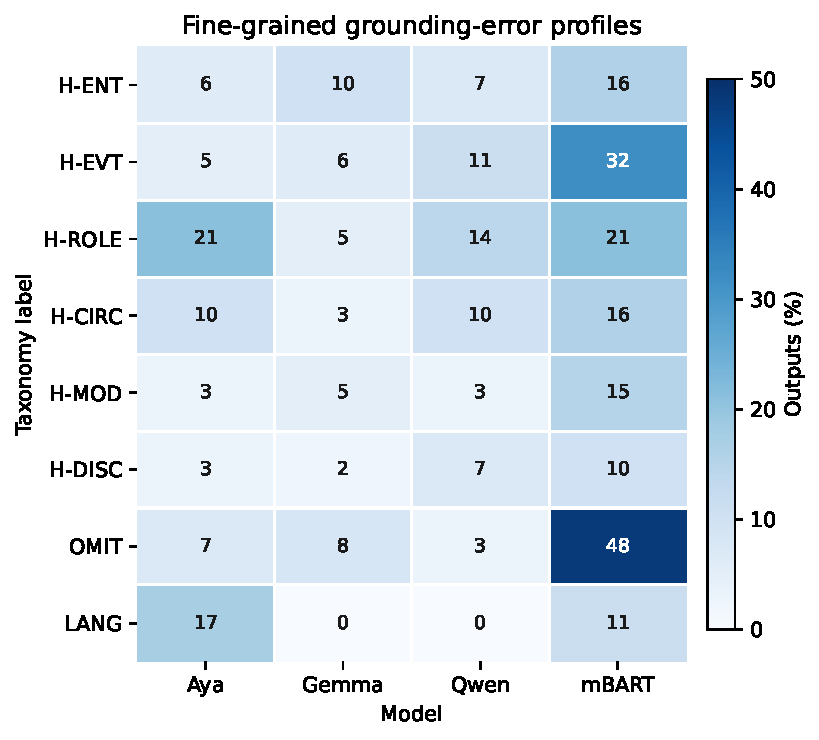
\includegraphics[width=0.98\columnwidth]{figures/all_models_taxonomy_heatmap.pdf}
\caption{Fine-grained taxonomy-label rates for the three SLMs and the mBART baseline. Each cell reports the percentage of a model's 100 outputs assigned the corresponding error label. Labels may overlap.}
\label{fig:slm-taxonomy-heatmap}
\end{figure}

\paragraph{Model-specific failure profiles.}
Aya had the lowest \textsc{No-Error} rate among the SLMs, with 43 hallucinated outputs, 7 omissions, and 17 language or format errors. Speaker-role hallucination was its dominant error type, appearing in 21 outputs. Most of Aya's \textsc{Lang} errors involved reproducing translated speaker turns instead of generating a summary. Gemma produced 63 error-free outputs and 29 outputs with hallucinations. Its most frequent error involved entities, and only 2 outputs received multiple labels. Qwen produced 58 error-free outputs and 39 outputs with hallucinations. Its errors were distributed across speaker roles, events, circumstances, and discourse relations. Qwen also produced the fewest omissions but the largest number of multi-label outputs among the three SLMs.

\paragraph{Taxonomy-specific patterns.}
Figure~\ref{fig:slm-taxonomy-heatmap} reports the fine-grained error label distribution for all four systems. Among the SLMs, speaker-role hallucination was the most frequent error, appearing in 40 outputs. These errors changed who performed an action, made a statement, offered assistance, or received an action. Entity and circumstantial hallucinations each appeared in 23 SLM outputs, while event hallucination appeared in 22 outputs. In contrast, mBART showed a different profile, with many omissions and event hallucinations in addition to role errors. Discourse and modality errors were less frequent for the SLMs, appearing in 12 and 11 outputs, respectively, but they also appeared in the mBART baseline.

\subsection{Automatic Evaluation}

Table~\ref{tab:automatic-results} presents the reference-based evaluation results. The supervised mBART baseline achieved the highest ROUGE and BERTScore values, while Gemma performed best among the zero-shot SLMs, with only small differences across the three SLMs.

The reference-based OmniScore dimensions showed a less uniform pattern. mBART received the highest clarity and plausibility scores but the lowest faithfulness score, whereas Aya obtained the highest faithfulness score among all systems.

Distributional statistics for all automatic metrics are provided in Appendix~\ref{sec:appendix-extended-eval}.

\section{Discussion}

\subsection{Relational Grounding Is the Main Challenge}

The dominant SLM failures were not primarily omissions or output-form failures. As Table~\ref{tab:grounding-results} shows, omission rates for the SLMs are only 0.03--0.08 and language/format error rates are 0.00--0.17, while hallucination rates are higher at 0.29--0.43. Figure~\ref{fig:slm-taxonomy-heatmap} further shows that these hallucinations concentrate in relation-sensitive categories: speaker-role errors appear in 40 SLM outputs, while entity, event, and circumstantial errors appear in 23, 22, and 23 outputs, respectively. This suggests that many hallucinations involve dialogue-relevant participants, events, or circumstances, but alter the relations among them.

Speaker-role hallucination illustrates this pattern: a summary may mention relevant participants or events but reverse who performed an action, made a request, offered assistance, or received it. Such errors are especially consequential in dialogue summarization, where requests, decisions, offers, and obligations depend on accurate speaker attribution across turns. Other frequent errors altered participants, events, pragmatic meaning, or contextual details, keeping summaries dialogue-related but structurally misaligned.

Modality and discourse errors were less frequent but still important because they changed whether an event was certain, intended, negated, agreed upon, or concluded. Faithful cross-lingual dialogue summarization therefore requires tracking not only entities and events, but also participant roles, epistemic status, and conversational outcomes across turns.


\subsection{Model Profiles Suggest Different Failure Modes}

The model-level profiles suggest that faithfulness failures arise through different pathways. Aya's errors were concentrated in speaker-role confusion and output-form problems, including cases where it reproduced translated speaker turns rather than generating a summary. This indicates that multilingual generation ability does not necessarily guarantee task control or successful compression into the required summary format.

Gemma and Qwen showed different SLM profiles. Gemma produced the most error-free outputs, with remaining errors that were relatively localized, often involving entities, omissions, events, or modality. Qwen produced fewer omissions but more distributed and multi-label errors, suggesting that a single misinterpretation can propagate across roles, events, circumstances, and discourse relations. These differences show why a single hallucination rate is insufficient for characterizing SLM reliability.

The mBART baseline exhibited a distinct failure mode. Despite being supervised, it showed many omissions and event hallucinations. This contrast reinforces the value of taxonomy-based analysis: it reveals not only whether a system fails, but how its failures are distributed across dialogue-semantic components.



\subsection{Automatic Metrics Are Auxiliary to Taxonomy-Based Diagnosis}

This contrast is clearest for the mBART baseline. mBART achieved the highest ROUGE-1, ROUGE-2, ROUGE-L, and BERTScore values, as well as the highest OmniScore clarity and plausibility scores. Under automatic evaluation alone, it would appear to be the strongest system. However, the manual taxonomy gives the opposite picture for source-grounded faithfulness: mBART had the lowest \textsc{No-Error} rate, the highest hallucination rate, and by far the highest omission rate. This shows that high reference similarity and fluent output form do not guarantee faithful representation of the source dialogue.

The discrepancy reflects a limitation of reference-based evaluation. An output can score well against a reference while omitting salient events, decisions, participant relations, or discourse outcomes. Conversely, an output may include source-supported details not selected by the reference, lowering reference similarity without necessarily indicating hallucination. Reference summaries are useful quality anchors, but they cannot directly determine whether a generated summary preserves the dialogue situation. Taxonomy-based diagnosis fills this gap by identifying which part of the dialogue meaning was altered, omitted, or unrealized.

\subsection{Implications for Relation-Aware Evaluation and Training}

Our findings suggest two directions for addressing relational grounding failures. First, relation-aware evaluation could represent the source dialogue and generated summary with event-centered structures that encode predicates, participant roles, circumstances, modality, and discourse outcomes. Such evaluation could test both whether summary relations are supported by the source and whether salient source relations are preserved, yielding category-specific diagnostics beyond reference similarity.

Second, the taxonomy can guide controlled hard negatives for contrastive or preference-based training. Starting from a faithful summary, minimally corrupted variants could swap participant roles, change events or circumstances, reverse modality, or alter decisions and discourse outcomes. Training models to distinguish faithful summaries from these category-specific corruptions may encourage preservation of dialogue-semantic relations across languages. These directions remain to be evaluated and are not claimed as contributions of the present diagnostic study.


\section{Conclusion}

We presented a taxonomy-based diagnosis of hallucination and faithfulness failures in zero-shot English-to-Chinese dialogue summarization with small language models. Across the three SLMs, failures were primarily relational: models often produced summaries involving dialogue-relevant content while altering speaker roles, events, circumstances, modality, or discourse outcomes. The taxonomy shows that SLM errors concentrate in dialogue-semantic components that require tracking participant roles, event structure, epistemic status, and conversational outcomes across turns. These findings support source-grounded taxonomy analysis as primary evidence for diagnosing SLM faithfulness, while automatic metrics serve as complementary indicators of target-summary quality.



\section{Limitations}

Our study is limited to 100 English-to-Chinese dialogues, three zero-shot SLMs, and three annotators, so the observed failure profiles may not generalize to other language directions, domains, prompts, or model families. The relatively small number of annotators may also make fine-grained labels sensitive to individual interpretation, particularly for overlapping or infrequent error categories. Because we do not include a monolingual control condition, the identified failures cannot be attributed exclusively to cross-lingual transfer, and the model-specific patterns should be interpreted as descriptive rather than causal. Finally, although all final labels were human-reviewed, the model-assisted first-pass annotation workflow may still introduce annotation bias.

\clearpage
\bibliography{custom}

\appendix
\section{Appendix}

\subsection{Data}
\label{sec:appendix-data}

XSAMSum pairs English messenger-style dialogues with abstractive English summaries and professional Chinese and German translations \citep{wang-etal-2022-clidsum}. We use the English dialogues as inputs and the Chinese summaries as references. Table~\ref{tab:xsamsum-statistics} reports the split-level statistics together with the 100-example evaluation subset. The subset is slightly shorter than the full test split in dialogue and reference length, while retaining similar average numbers of turns and speakers.

\begin{table}[H]
\centering
\footnotesize
\setlength{\tabcolsep}{4pt}
\begin{tabular}{lrrrr}
\hline
Metric & Train & Dev & Test & Eval. subset \\
\hline
Dialogues         & 14{,}732 & 818   & 819   & 100 \\
Turns             & 11.17    & 10.83 & 11.25 & 10.87 \\
Speakers          & 2.39     & 2.39  & 2.36  & 2.43 \\
Dialogue words    & 93.79    & 91.64 & 95.51 & 88.21 \\
En. summary words & 20.32    & 20.28 & 20.02 & 18.62 \\
Zh. summary chars & 35.88    & 35.99 & 35.05 & 33.18 \\
\hline
\end{tabular}
\caption{XSAMSum statistics. Except for the number of dialogues, values are averages. Dialogue and English-summary lengths use whitespace-delimited words; Chinese-summary length counts non-whitespace characters. The evaluation subset is sampled from the test split with seed 42.}
\label{tab:xsamsum-statistics}
\end{table}

\subsection{Model Details}
\label{sec:appendix-model-details}

\paragraph{mBART fine-tuning.}

Our supervised baseline is initialized from \texttt{facebook/mbart-large-50-many-to-many-mmt} \citep{liu-etal-2020-multilingual-denoising,tang-etal-2021-multilingual}. It is fine-tuned end to end to map an English XSAMSum dialogue directly to its Chinese reference summary, without an intermediate translation stage.

Training uses Hugging Face's \texttt{Seq2SeqTrainer} on a Google Colab instance with one NVIDIA A100 40GB GPU. We optimize with Adafactor for five epochs using mixed precision and gradient checkpointing, and select the checkpoint with the best validation \texttt{ROUGE-Lsum}. The tokenizer source and target languages are set to \texttt{en\_XX} and \texttt{zh\_CN}, respectively, and generation is forced to begin with the Chinese language token. Table~\ref{tab:mbart-training} summarizes the main settings.

\begin{table}[H]
\centering
\footnotesize
\setlength{\tabcolsep}{4pt}
\begin{tabularx}{\columnwidth}{@{}lX@{}}
\hline
Setting & Value \\
\hline
Maximum input length & 768 tokens \\
Maximum target length & 64 tokens \\
Epochs & 5 \\
Learning rate & $2\times10^{-5}$ \\
Per-device batch size & 4 \\
Gradient accumulation & 6 steps \\
Effective batch size & 24 \\
Optimizer & Adafactor \\
Precision & Mixed precision \\
Checkpoint selection & Validation \texttt{ROUGE-Lsum} \\
Decoding & Beam search with 5 beams \\
Source / target language & \texttt{en\_XX} / \texttt{zh\_CN} \\
Hardware & NVIDIA A100 40GB \\
\hline
\end{tabularx}
\caption{mBART fine-tuning and decoding configuration.}
\label{tab:mbart-training}
\end{table}

\paragraph{SLM direct inference.}

We evaluate the three instruction-tuned SLMs in the same zero-shot direct setting. Each model receives the English dialogue and generates a Simplified Chinese summary without demonstrations, intermediate translation, or task-specific fine-tuning. The models are run locally through Ollama with a temperature of 0.2, an 8,192-token context window, a maximum of 1,024 generated tokens, and explicit reasoning output disabled.

\begin{itemize}
    \item \textbf{Qwen 3.5 9B.} We use the Ollama model \texttt{qwen3.5:9b}, an instruction-tuned Qwen-family model selected for its multilingual understanding and text-generation capabilities \citep{qwenteam2026qwen35omnitechnicalreport}.

    \item \textbf{Gemma 4 E4B.} We use \texttt{gemma4:e4b}, an efficient instruction-tuned model from the Gemma family, as a lightweight multilingual baseline \citep{gemma4_2026}.

    \item \textbf{Aya Expanse 8B.} We use \texttt{aya-expanse:8b}, a multilingual instruction-tuned model designed to support generation across 23 languages \citep{dang2024ayaexpansecombiningresearch}.
\end{itemize}

\subsection{Direct Prompt}
\label{sec:appendix-direct-prompt}

All three SLMs receive the prompt template in Figure~\ref{fig:direct-prompt}, with \texttt{\{dialogue\}} replaced by the speaker-prefixed English input.

\begin{figure}[H]
\centering
\fbox{%
\begin{minipage}{0.92\columnwidth}
\small\ttfamily\raggedright
You are an expert English-Chinese bilingual speaker. Given an English dialogue, please write a concise Simplified Chinese summary. Output only the summary, without titles or markdown.

\medskip
English dialogue:\par
\{dialogue\}

\medskip
Chinese summary:
\end{minipage}%
}
\caption{Direct prompt template used for zero-shot SLM inference.}
\label{fig:direct-prompt}
\end{figure}

\FloatBarrier

\subsection{Relation to Prior Dialogue-Summarization Taxonomies}
\label{sec:appendix-taxonomy-comparison}

Table~\ref{tab:taxonomy-comparison} summarizes approximate correspondences between our categories and the dialogue-summarization taxonomies of \citet{tang-etal-2022-confit} and \citet{wang-etal-2022-analyzing}. The categories are not exact equivalents: our scheme is organized by the dialogue-semantic relation affected and is applied by comparing each cross-lingual output directly with its source dialogue.

\begin{table*}[t]
\centering
\scriptsize
\setlength{\tabcolsep}{4pt}
\begin{tabularx}{\textwidth}{@{}lXXX@{}}
\toprule
Our category & Tang et al. (2022) & Wang et al. (2022) & Primary emphasis in our taxonomy \\
\midrule
\textsc{H-Ent}  & Object / Wrong Reference & Subject--Object / Pronoun & Entity identity, separated from event and participant role \\
\textsc{H-Evt}  & --- & Hallucination & Added, changed, or fabricated event \\
\textsc{H-Role} & Wrong Reference & Subject--Object & Actor--recipient--speaker relation \\
\textsc{H-Circ} & Circumstantial & Particulars & Time, place, quantity, condition, or schedule \\
\textsc{H-Mod}  & Negation / Tense / Modality & Negation & Negation, uncertainty, intention, obligation, or modal force \\
\textsc{H-Disc} & --- & Other & Cause, contrast, order, decision, agreement, or outcome \\
\textsc{Omit}   & Missing Information & --- & Salient information absent from the output \\
\textsc{Lang}   & --- & --- & Cross-lingual language, format, or task-fulfillment failure \\
\bottomrule
\end{tabularx}
\caption{Approximate correspondence between our taxonomy and prior factual-error taxonomies for dialogue summarization. A dash indicates that the prior work has no directly corresponding standalone category; it does not imply that the broader phenomenon is entirely absent.}
\label{tab:taxonomy-comparison}
\end{table*}

\FloatBarrier

\subsection{Annotation Workflow}
\label{sec:appendix-annotation-workflow}

For the dialogue-semantic grounding analysis, we used a model-assisted first-pass annotation workflow. An annotation model was used only to propose candidate labels for each generated summary; it was not used as an evaluated summarization system and was not treated as the final annotator. Each candidate label was subsequently reviewed against the English source dialogue, the Chinese reference summary, the generated Chinese summary, and the taxonomy definitions in Table~\ref{tab:taxonomy}.

The review prioritized source-grounded faithfulness: a hallucination label was assigned only when the generated summary introduced or altered information relative to the dialogue, while \textsc{Omit} and \textsc{Lang} captured missing salient information and output-form failures, respectively. Multi-label annotations were allowed when a single summary contained multiple independent error types. Three annotators participated in the review process; each output was reviewed by at least one annotator, and uncertain cases were discussed before finalizing the label.

\FloatBarrier

\subsection{Extended Automatic Evaluation}
\label{sec:appendix-extended-eval}

Table~\ref{tab:reference-metric-distributions} and Table~\ref{tab:omniscore-distributions} supplement the mean scores in Table~\ref{tab:automatic-results} with dispersion, median, range, and 95\% confidence intervals. Each model contributes 100 outputs.

\begin{table*}[t]
\centering
\scriptsize
\setlength{\tabcolsep}{5pt}
\begin{tabular}{llrrrr}
\hline
Model & Metric & SD & Median & Min--Max & 95\% CI \\
\hline
Aya   & ROUGE-1   & 10.58 & 24.28 & 5.26--51.28   & 24.46--28.60 \\
Aya   & ROUGE-2   & 6.81  & 5.97  & 0.00--28.28   & 6.55--9.22 \\
Aya   & ROUGE-L   & 9.02  & 19.23 & 5.26--51.28   & 19.07--22.60 \\
Aya   & BERTScore & 4.60  & 70.33 & 59.70--83.88  & 69.21--71.02 \\
Gemma & ROUGE-1   & 11.35 & 30.28 & 0.00--61.54   & 28.05--32.50 \\
Gemma & ROUGE-2   & 7.51  & 7.37  & 0.00--34.15   & 6.85--9.79 \\
Gemma & ROUGE-L   & 10.30 & 24.32 & 0.00--54.55   & 21.66--25.70 \\
Gemma & BERTScore & 5.58  & 71.06 & 57.16--84.79  & 69.76--71.94 \\
Qwen  & ROUGE-1   & 11.12 & 27.09 & 3.88--53.85   & 26.17--30.53 \\
Qwen  & ROUGE-2   & 8.27  & 5.27  & 0.00--48.48   & 6.00--9.24 \\
Qwen  & ROUGE-L   & 10.03 & 21.05 & 3.88--51.95   & 20.45--24.38 \\
Qwen  & BERTScore & 4.72  & 70.32 & 56.95--83.35  & 69.55--71.40 \\
mBART & ROUGE-1   & 19.06 & 37.97 & 8.33--100.00  & 38.21--45.68 \\
mBART & ROUGE-2   & 20.10 & 12.50 & 0.00--100.00  & 14.16--22.04 \\
mBART & ROUGE-L   & 18.62 & 31.17 & 8.33--100.00  & 31.21--38.50 \\
mBART & BERTScore & 8.40  & 76.16 & 60.94--100.00 & 76.00--79.29 \\
\hline
\end{tabular}
\caption{Distributional statistics for ROUGE and BERTScore. Mean values are reported in Table~\ref{tab:automatic-results}.}
\label{tab:reference-metric-distributions}
\end{table*}

\begin{table*}[t]
\centering
\scriptsize
\setlength{\tabcolsep}{5pt}
\begin{tabular}{llrrrr}
\hline
Model & OmniScore dimension & SD & Median & Min--Max & 95\% CI \\
\hline
Aya   & Informativeness & 0.58 & 3.31 & 2.00--4.74 & 3.15--3.38 \\
Aya   & Clarity         & 0.37 & 3.99 & 2.95--4.93 & 3.95--4.09 \\
Aya   & Plausibility    & 0.37 & 4.02 & 2.86--4.93 & 3.97--4.12 \\
Aya   & Faithfulness    & 0.51 & 3.09 & 2.15--4.74 & 3.07--3.27 \\
Gemma & Informativeness & 0.56 & 3.13 & 2.01--4.66 & 3.06--3.28 \\
Gemma & Clarity         & 0.32 & 3.94 & 2.87--4.93 & 3.88--4.01 \\
Gemma & Plausibility    & 0.31 & 3.95 & 2.89--4.93 & 3.94--4.06 \\
Gemma & Faithfulness    & 0.42 & 2.96 & 2.03--3.87 & 2.88--3.04 \\
Qwen  & Informativeness & 0.50 & 3.30 & 1.87--4.31 & 3.12--3.32 \\
Qwen  & Clarity         & 0.26 & 3.90 & 3.17--4.72 & 3.83--3.93 \\
Qwen  & Plausibility    & 0.26 & 3.97 & 3.09--4.77 & 3.92--4.02 \\
Qwen  & Faithfulness    & 0.34 & 3.01 & 2.01--3.73 & 2.94--3.07 \\
mBART & Informativeness & 0.68 & 2.85 & 1.53--4.84 & 2.83--3.10 \\
mBART & Clarity         & 0.41 & 4.22 & 3.36--4.93 & 4.16--4.32 \\
mBART & Plausibility    & 0.42 & 4.13 & 3.35--4.94 & 4.08--4.25 \\
mBART & Faithfulness    & 0.66 & 2.79 & 1.65--4.74 & 2.79--3.05 \\
\hline
\end{tabular}
\caption{Distributional statistics for the four reference-based OmniScore dimensions. Mean values are reported in Table~\ref{tab:automatic-results}.}
\label{tab:omniscore-distributions}
\end{table*}

\subsection{Overall SLM Label and Outcome Distributions}
\label{sec:appendix-overall-taxonomy}

Figure~\ref{fig:overall-taxonomy-label-counts} reports the overall occurrence counts for each taxonomy label across the 300 SLM outputs, excluding the mBART baseline. Figure~\ref{fig:overall-semantic-outcome} summarizes the corresponding binary semantic outcome. Multi-label outputs contribute once to each assigned label.

\begin{figure}[H]
\centering
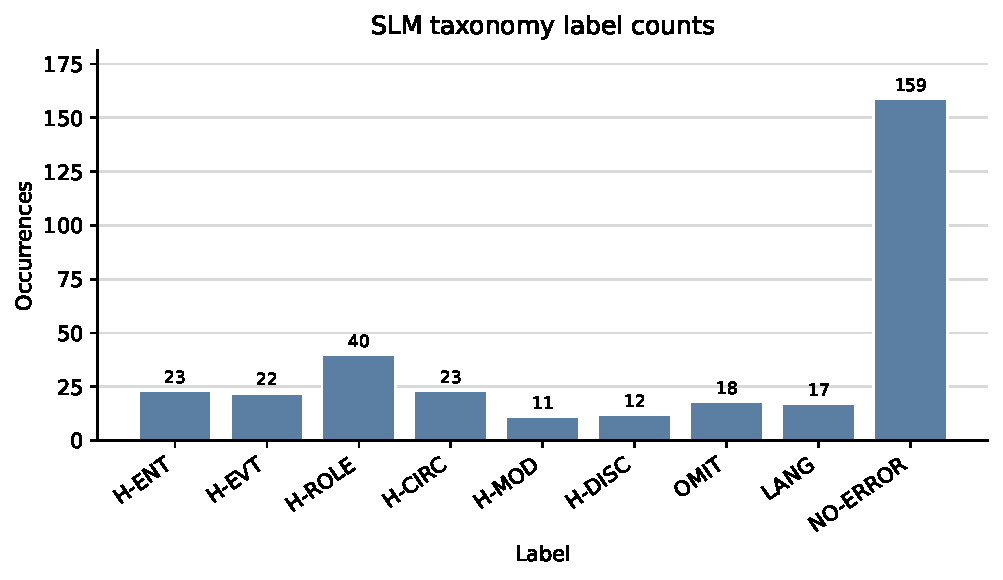
\includegraphics[width=0.98\columnwidth]{figures/overall_taxonomy_label_counts.pdf}
\caption{Overall taxonomy-label occurrence counts across the three SLMs, excluding mBART. Multi-label outputs are decomposed into individual label occurrences.}
\label{fig:overall-taxonomy-label-counts}
\end{figure}

\begin{figure}[H]
\centering
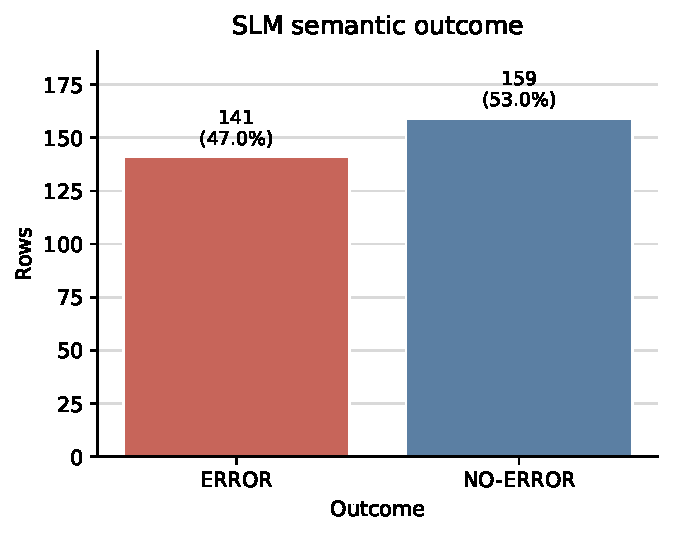
\includegraphics[width=0.82\columnwidth]{figures/overall_semantic_outcome.pdf}
\caption{Overall semantic outcome counts across the three SLMs, excluding mBART. Outputs labeled \textsc{No-Error} are counted as no-error cases; all other outputs are counted as error cases.}
\label{fig:overall-semantic-outcome}
\end{figure}

\end{document}
